\title{Atomic modeling of Argon}
\author{
        Andreas V. Solbr\aa \\
                University of Oslo\\
		 Department of Computational Physics
}

\documentclass[12pt]{article}
\usepackage{amsmath}
\usepackage{fullpage}
\usepackage{amsthm}
\usepackage{amsfonts}
\usepackage{graphicx}
\usepackage[english]{babel}
\usepackage[T1]{fontenc}
\usepackage{subfigure}
\usepackage{epstopdf}
\usepackage[hyphens]{url}
\usepackage{gensymb}
\usepackage{verbatim}
%\usepackage{slashed}
\usepackage{amssymb}
\usepackage{amsfonts}
%\usepackage{caption}
%\usepackage{subcaption}
\newtheorem{thm}{Theorem}

%% Define a new 'leo' style for the package that will use a smaller font.
\makeatletter
\def\url@leostyle{%
  \@ifundefined{selectfont}{\def\UrlFont{\sf}}{\def\UrlFont{\small\ttfamily}}}
\makeatother
%% Now actually use the newly defined style.
\urlstyle{leo}


%\usepackage[utf8]{inputenc}
%\usepackage{textcomp}
%\usepackage[T1]{fontenc}




\newcommand{\Fig}[1]{Figure~\ref{#1}}
\newcommand{\fig}[1]{figure~\ref{#1}}
\newcommand{\eq}[1]{equation~\ref{#1}}
\newcommand{\Eq}[1]{Equation~\ref{#1}}

% Shortcuts for including equations
\newcommand{\beq}{\begin{equation}}
\newcommand{\eeq}{\end{equation}}
\def\ivec{\textbf{i}}
\def\jvec{\textbf{j}}
\def\kvec{\textbf{k}}
\def\uvec{\textbf{u}}
\def\vvec{\textbf{v}}
\def\xvec{\textbf{x}}
\def\rvec{\textbf{r}}
\def\Rvec{\textbf{R}}
\def\Fvec{\textbf{F}}
\def\S{\hat{S}}
\def\Svec{\hat{\textbf{S}}}
\def\H{\hat{H}}
\def\ro{\hat{\rho}}
\def\trace{\operatorname{Tr}}
\def\Lop{\hat{L}}
\def\etavec{\hat{\boldsymbol\eta}}
\def\X{\hat{X}}
\def\Y{\hat{Y}}
\def\etaop{\hat{\eta}}
\def\A{\hat{\textbf{A}}}
\def\B{\textbf{B}}
\def\aop{\hat{a}}
\def\aopd{\hat{a}^\dagger}
\def\bop{\hat{b}}
\def\bopd{\hat{b}^\dagger}




% Document formatting
\setlength{\parindent}{0mm}
\setlength{\parskip}{1.5mm}

% Hyper refs
\usepackage[pdftex,colorlinks,breaklinks]{hyperref}
\usepackage{listings}
\usepackage{color}
\usepackage{textcomp}
\definecolor{listinggray}{gray}{0.9}
\definecolor{lbcolor}{rgb}{0.9,0.9,0.9}
\definecolor{pink}{RGB}{255, 119, 255}
\lstset{
	backgroundcolor=\color{lbcolor},
	tabsize=4,
	rulecolor=,
	language=c++,
        basicstyle=\scriptsize,
        upquote=true,
        aboveskip={1.5\baselineskip},
        columns=fixed,
        showstringspaces=false,
        extendedchars=true,
        breaklines=true,
        prebreak = \raisebox{0ex}[0ex][0ex]{\ensuremath{\hookleftarrow}},
        frame=single,
        showtabs=false,
        showspaces=false,
        showstringspaces=false,
        identifierstyle=\ttfamily,
        keywordstyle=\color[rgb]{0,0,1},
        commentstyle=\color[rgb]{0.133,0.545,0.133},
        stringstyle=\color[rgb]{0.627,0.126,0.941},
	title=\lstname
}

\newcounter{subproject}
\renewcommand{\thesubproject}{\alph{subproject}}
\newenvironment{subproj}{
\begin{description}
\item[\refstepcounter{subproject}(\thesubproject)]
}{\end{description}}
\date{\today}

\begin{document}
 \maketitle
 \begin{abstract}
  The goal of this project is to gain experience with the methods used in simulations of molecular dynamics. In the project we will use Argon atoms as a prototype, and measure the different physical properties of our model.
 \end{abstract}
 
 \section{Setting up a system}
 We start by placing the particles in a face centered cube formation, as shown in figure \ref{fig:1}. We can describe this by one of the corners of the cube, and the relative position of the other particles in the grid. The positions of the cells in a $N \times N \times N$ lattice are therefore 
 \begin{equation}
  \Rvec_{i,j,k} = i\hat{\uvec}_1 + j\hat{\uvec}_2 + k\hat{\uvec}_3
 \end{equation}
 where the basic unit vectors are the cartesian vectors multiplied by the length $b$ of the unit cell,and the relative positions of the atoms in the cell  are 
 \begin{align}
  \rvec &= 0 \hat{i} + 0 \hat{j} + 0 \hat{k} \\
  & = {b \over 2} \hat{i} + {b \over 2} \hat{j} + 0 \hat{k} \\
  & = 0 \hat{i} + {b \over 2} \hat{j} + {b \over 2} \hat{k} \\
  & = {b\over 2} \hat{i} + 0 \hat{j} + {b\over 2} \hat{k}
 \end{align}
for solid Argon, the lattice constant is $b = 5.260$ \AA. The code for this can be found in the function \verb setPosFFC()  in the file \verb system.cpp  in the source code located at \verb www.github.com/andreavs/fys4460 . 

 
  \begin{figure}
\centering
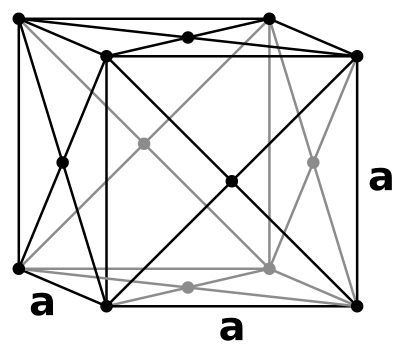
\includegraphics[width=8cm]{facecenteredcube.png}
\caption{\label{fig:1} The figure shows a face centered cube}
\end{figure}
 
 
 \subsection{setting initial velocities}
 From statistical physics we know that that at equilibrium temperature $T$, the velocities are given by the Boltzmann distribution, which mean that the individual components are normally distributed. The standard deviation is $\sqrt{k_B T/m}$ where $m$ is the mass of the atom, $T$ is the temperature of the system and $k_B$ is the Boltzmann constant. To avoid any drift in the system, we can calculate the the total drift in the system, and then subtract the average drift from each particle. The code for this can be found in the function \verb setVelNormal()  in \verb system.cpp .
 
\section{Time evolution of the system}
We use the symplectic and numerically stable velocity Verlet algorithm to integrate particle motion. Even though this integrator is simple, it is time reversible and provides excellent energy conservator. 

For each particle $i$, the steps are as follows:
\begin{align}
 \vvec_i(t+\Delta t/2) &= \vvec_i(t) + {\Fvec_i(t) \over 2m} \Delta t \\
 \rvec_i(t + \Delta t) &= \rvec_i(t) + \vvec_i(t \Delta t/2 )\Delta t \\
 \Fvec_i(t+\Delta t) &= -\nabla_i U_i ({\rvec(t+\Delta t)}) \\
 \vvec_i(t+\Delta t) &= \vvec_i(t+\Delta t/2) + {\Fvec_i(t+\Delta t) \over 2m} \Delta t
\end{align}

This is implemented in the function \verb timeEvolve()  in \verb system.cpp . If we implement this as it stand using $U_i = 0$ as a first test, what we will see is that the particles spread out into the empty space with their initial velocity. We do not want this behaviour. As we want to look at the statistics of our system, we can rather impose periodic boundary conditions. 

\subsection{Periodic boundary conditions}
We want to keep our particle density constant. One way to achieve this is to say that if a particle travels beyond the edge of one of the walls in the system, is simply enters the system on the oposite side. A good way to implement this is to impose this requirement right after the position step in the integrator. This requirement is implemented in the method \verb setPeriodicBoundaries()  in  \verb system.cpp . 

Implementing this let's us see the particles move within their assigned box, but they still move in a straight line with their initial velocities as there are no forces acting on them. In the next subsection we implement a simple force model.

\subsection{Forces}
We use a Lennard-Jones potential for the interatomic interactions. The Lennard Jones potential has the following form:
\begin{equation}
 U(r) = 4\epsilon\left[ \left({\sigma \over r}\right)^{12} - \left({\sigma \over r}\right)^6 \right]
\end{equation}
where $r$ is the distance between the atoms. For Argon optimal values of the parameters are: 
\begin{equation}
 {\epsilon \over k_B} = 119.7 {\rm K}, \quad \sigma = 3.405 {\text{\AA .}}
\end{equation}
From this we find the force between particle $i$ and $j$ to be
\begin{align}
 \Fvec(\rvec_{ij}) & = -\nabla U(r_{ij}) \\
 & = -{\partial U \over \partial r_{ij}} \hat{\rvec}_{ij} \\
 & = {24\epsilon \over r} \left[ 2\left( {\sigma \over r} \right)^{12} - \left( {\sigma \over r_{ij}} \right)^{6} \right]\hat{\rvec}_{ij}
\end{align}
where $\rvec_{ij} = \rvec_j - \rvec_i$, $r_{ij} = |\rvec_{ij}|$ and $\hat{\rvec}_{ij} = \rvec_{ij}/r_{ij}$. We may note that the equilibrium distance is $r = 2^{1/6}\sigma \approx 1.122\sigma$. This is a good time to choose appropriate units for our simulation. Introducing the dimensionless variable $\tilde{r} = r/\sigma$, and meassuring energy in units of $\epsilon$, we do not have to pay attention to these in our program.

We want our forces to adhere to our periodic boundaries, so that we calculate the distance to the other atom using the minimum image convention, as illustrated in figure \ref{fig:2}. To a point, we let the distance in the $x$ direction become $\min \{ |x_i - x_j - L|, |x_i - x_j|, |x_i - x_j + L| \}$ and so on. 

  \begin{figure}
\centering
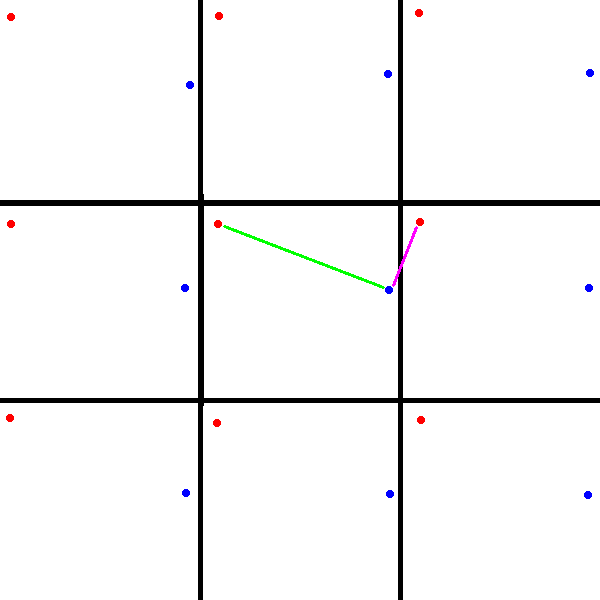
\includegraphics[width=8cm]{minimalimage.png}
\caption{\label{fig:2} The figure illustrates the minimal image convention. The middle box is our system, and the outlying boxes are the periodic extensions. Withour the minimal image convention, the green line would be used as the distance. However, the purple line is a better choice, so this is used instead.}
\end{figure}

This force model is implemented in the function \verb singlePairForces() , which is called by the function \verb calculateForcesLJMIC() , whose job it is to run over all the pairs of particles in the system. This is done using Newton's third law so there are no superflous calculations. This operation, however, still scales as $~N^2$ where $N$ is the number of particles, which quickly becomes far to time consuming for large systems. In the next section we will look into how we can adress this. However, we know have a working model for simulating Argon, and it is worthwhile to simulate this using software such as VMD or Ovito. An example of the latter is shown in figure \ref{fig:3}, where the an $8\times 8 \times 8$ grid is simulated using a starting temperature of 100 Kelvin. We see that after some initial scattering due to the initial velocities, the system relaxes into a solid grid. 

  \begin{figure}
\centering
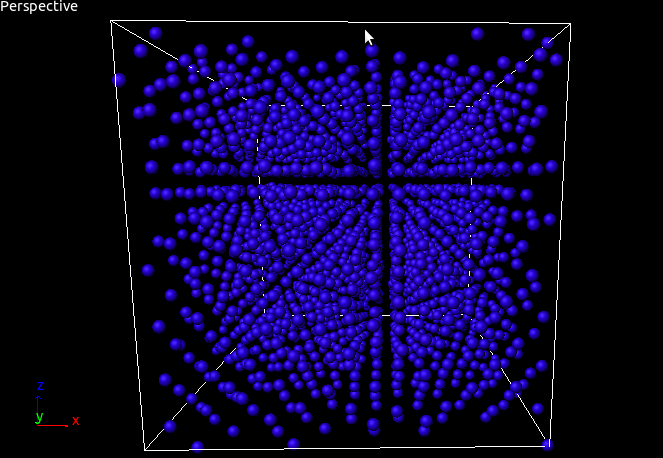
\includegraphics[width=12cm]{simpleovito.png}
\caption{\label{fig:3} The figure shows a simple animation of our Argon system in Ovito.}
\end{figure}


\section{Speed up: Computation cells}
The force calculations are very time consuming. We want to improve this by negleting  force terms for particles that are very far apart. The Lennard-Jones potential can be neglected for distances longer than $r_{{\rm cut}} = 3\sigma$. A fairly straight forward way to this is to divide our system into several cells, as illustrated in figure \ref{fig:4}. We then let each cell calculate forces within itself and its 26 neighbouring cells. 

We may want to implement Newton's third law in this system, and one way to do this is to only let one cell point to 13 of its neighbours, and let the 13 remaining neighbours point to the cell, so there are no redundant calculations. This is illustrated in figure \ref{fig:5}. 

The atoms can be stored in the cells using linked lists. The implementation of computation cells can be found in the functions \verb placeAtomsInCells()  and \verb calculateForcesCellsLJMIC() , as well as the class \verb Cell . The neighbour lists are made in the constructor of the system.

  \begin{figure}
\centering
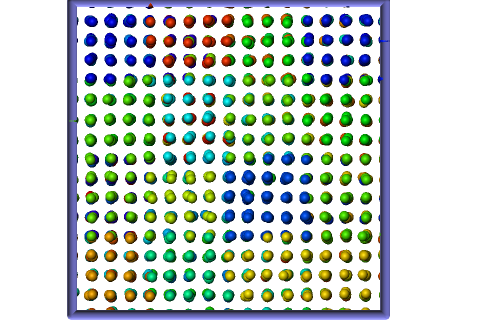
\includegraphics[width=10cm]{cellexample.png}
\caption{\label{fig:4} In this figure each computation cell is assigned a random color, and and the particles are colored by their cell.}
\end{figure}

  \begin{figure}
\centering
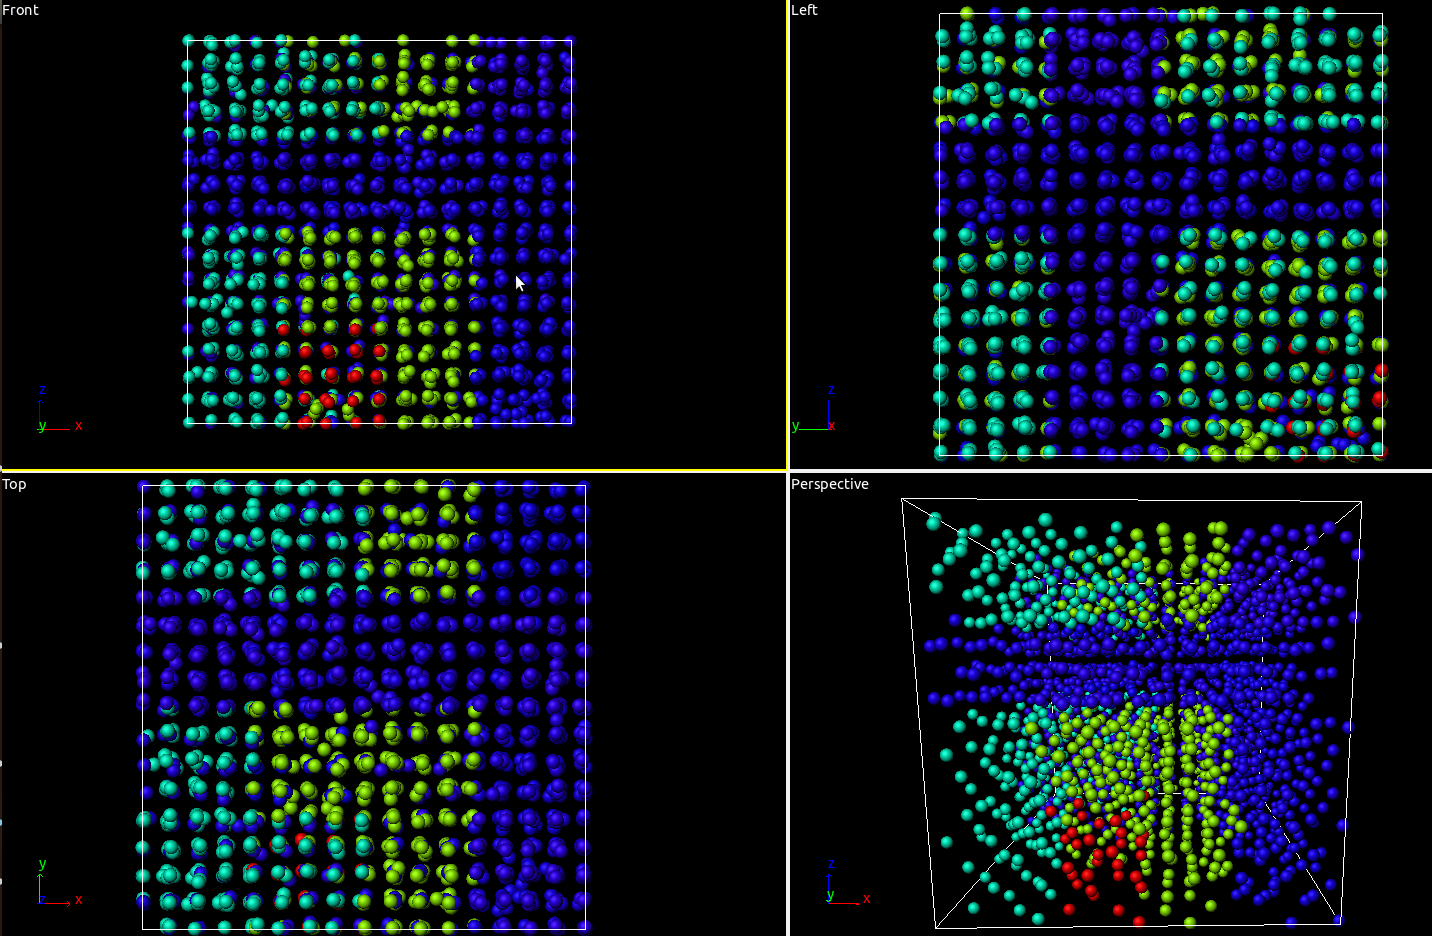
\includegraphics[width=16cm]{neighbourcells.png}
\caption{\label{fig:5} The figure illustrates the one-way neighbours. The red cell is the main character, the green cells are the neighbours it points to, and the cyan cells point to the main cell. The different pictures are different orientations of the same system.}
\end{figure}

\section{Macroscopic Observables}
We can test the quality of our model by meassuring different physical properties of the system, and compare the results with the predictions from statisical mechanics. The rest of the report will be dedicated to this.

\subsection{Maxwell-Boltzmann distribution at equilibrium}
According to the 2nd law of thermodynamics and entropy considerations, the velocity distribution will evolve into a Maxwell-Boltzmann distribution independent of the initial conditions. We can test this by letting the initial velocity components of the particles be uniformly distributed, and making histograms of the velocities at different times. This is shown if figure \ref{fig:6}. We see that the distribution tend to a Maxwell-Boltzmann distribution.

\begin{figure}[ht]
\centering
\subfigure[initial x-component of the velocity]{
	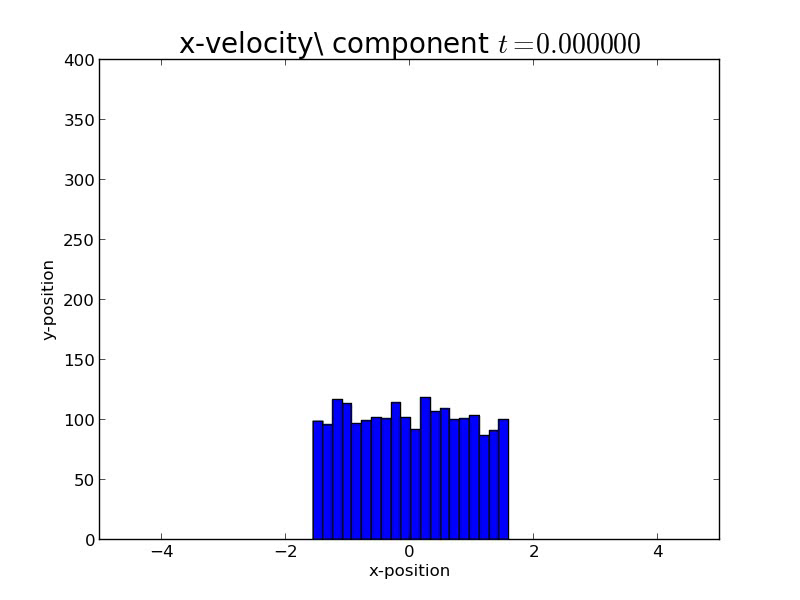
\includegraphics[width=7cm]{firstxvel.png}
	\label{fig:subfig1}
}
\subfigure[x-component of the velocity at a later time]{
	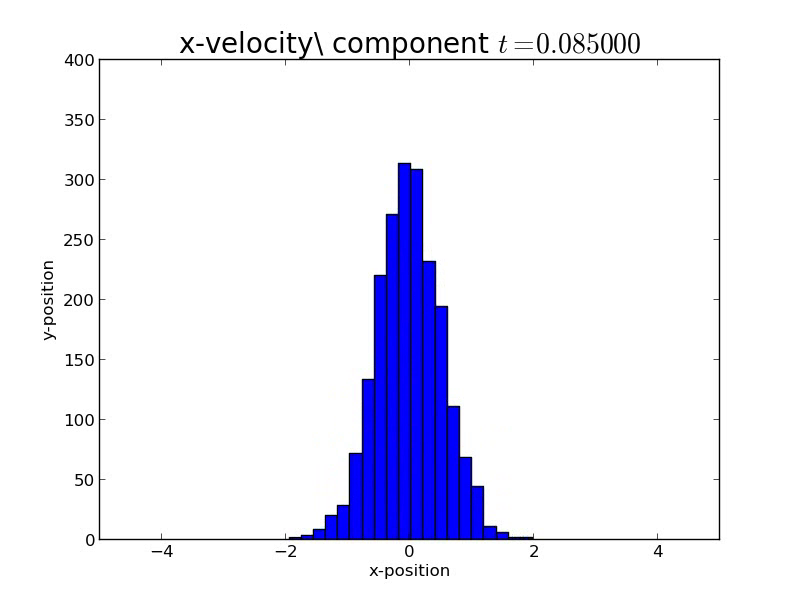
\includegraphics[width=7cm]{laterxvel.png}
	\label{fig:subfig2}
}
\subfigure[Initial velocity distribution]{
	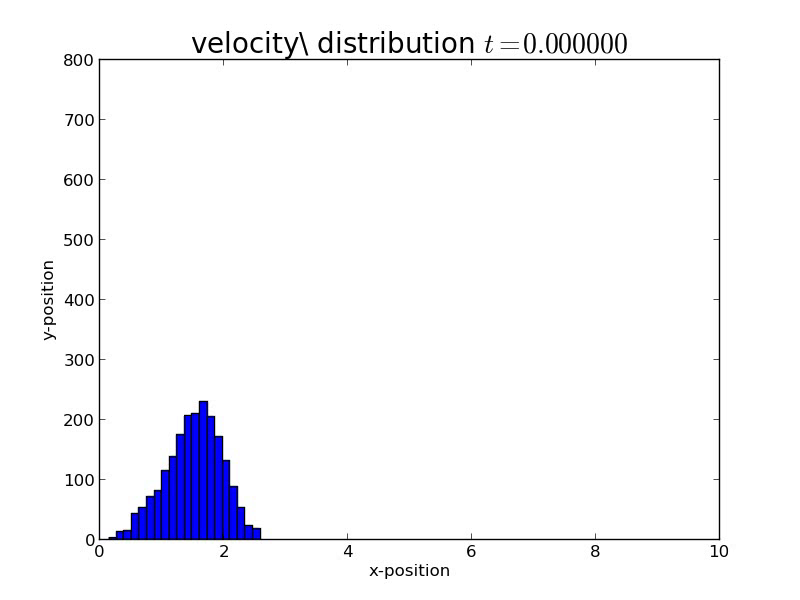
\includegraphics[width=7cm]{firstvel.png}
	\label{fig:subfig3}
}
\subfigure[Velocity distribution at a later time]{
	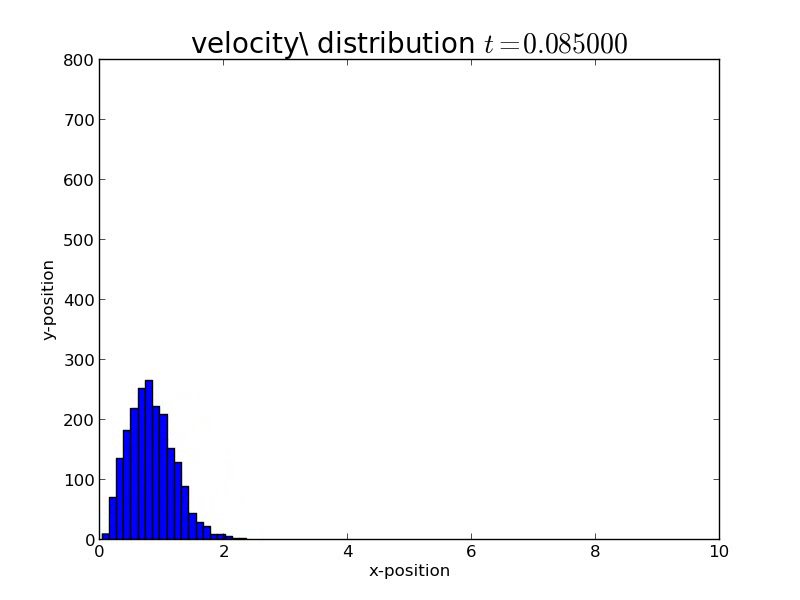
\includegraphics[width=7cm]{latervel.png}
	\label{fig:subfig3}
}
\caption[Optional caption for list of figures]{The plots show the distribution of the x-component and the size of the velocities a initially and after the system has settled.}
\label{fig:6}
\end{figure}

\subsection{Energy, temperature and pressure of the system}
From the velocities and the potential, we can find the kinetic, potential and total energy of the system. From this, we can use 
\begin{equation}
 \langle E_k \rangle = {3\over 2}Nk_B T 
\end{equation}
to estimate the temperature of the system, and we can meassure the pressure as 
\begin{equation}
 P = \rho k_B T + {1 \over 3V}\sum_{i<j} \Fvec_{ij} \cdot \rvec_{ij},
\end{equation}
which is valid for the micro-canonical ensemble. The results for a are shown for a starting temperature of 300 Kelvin in figures \ref{fig:7} and \ref{fig:8}, with a time step of 0.005 (in MD units). We see that the temperature quickly drops, before becoming stable. The total energy fluctuations are alsmost are small. It is interesting to see how the fluctuations vary as a function of the time step. Table \ref{tab:1} shows the variance of the energies for different values of $\Delta t$. 

\begin{table}
 \centering
 \begin{tabular}{|l|l|}
  \hline
  $\Delta t$ & Var($E$) \\
  \hline
  0.001 & 0.0197 \\ 
  0.005 & 0.1208 \\
  0.01 & 1.6565 \\
  \hline
 \end{tabular}
\caption{\label{tab:1} The table shows a the variance in energy for a few values of $\Delta t$. It looks as the fluctuations become smaller as $\Delta t$ decreases.}
\end{table}


  \begin{figure}
\centering
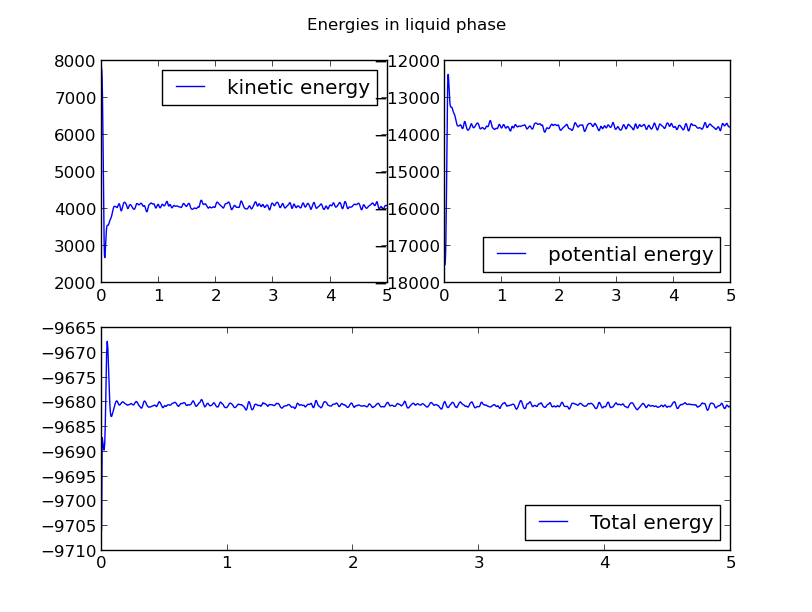
\includegraphics[width=10cm]{simpleenergies.png}
\caption{\label{fig:7} The figure shows the kinetic, potential and total energy of the system as a function of time, using an initial temperature of 300 Kelvin and a time step of 0.005 in MD units.}
\end{figure}

  \begin{figure}
\centering
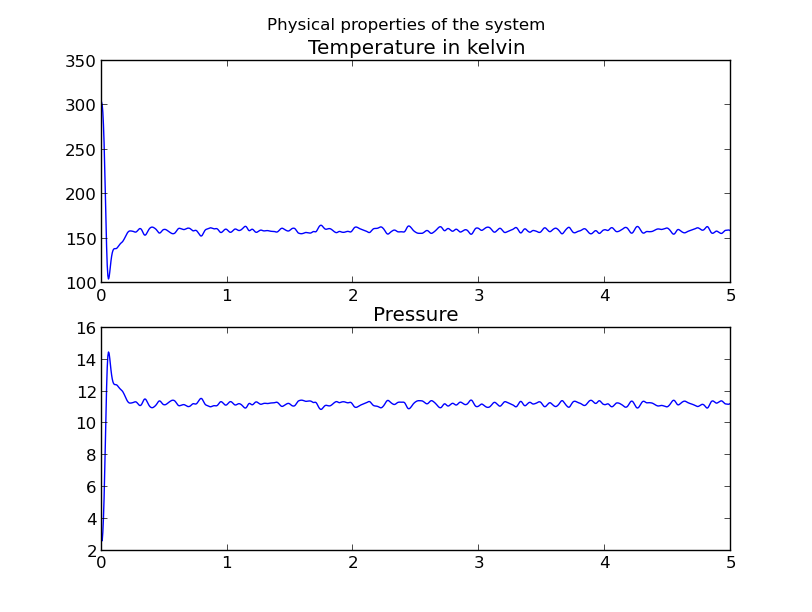
\includegraphics[width=10cm]{simplephysproperties.png}
\caption{\label{fig:8} The figure shows the temperature and pressure of the system using an initial temperature of 300 Kelvin and a time step of 0.005 in MD units}
\end{figure}

Later we will implement a thermostat to our system, which will allow us to change the temperature of the system, and so we can plot the pressure as a function of the temperature. This is shown in figure \ref{fig:9}. We see that there at one point is a sudden change in pressure while the temperature is relatively constant, and we can interpret this as a phase transition.

\begin{figure}[ht]
\centering
\subfigure[Pressure as a function of Temperature]{
	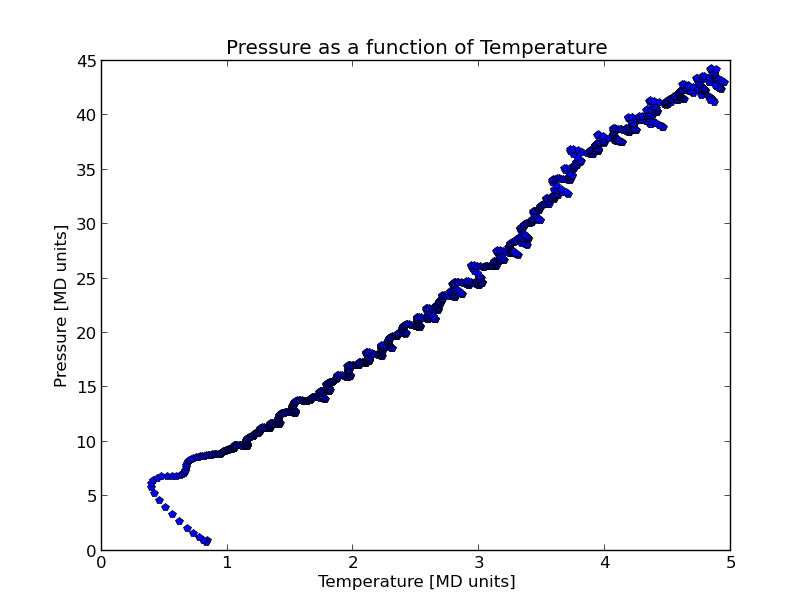
\includegraphics[width=7cm]{phasetransition.png}
	\label{fig:subfig13}
}
\subfigure[Mean square displacement]{
	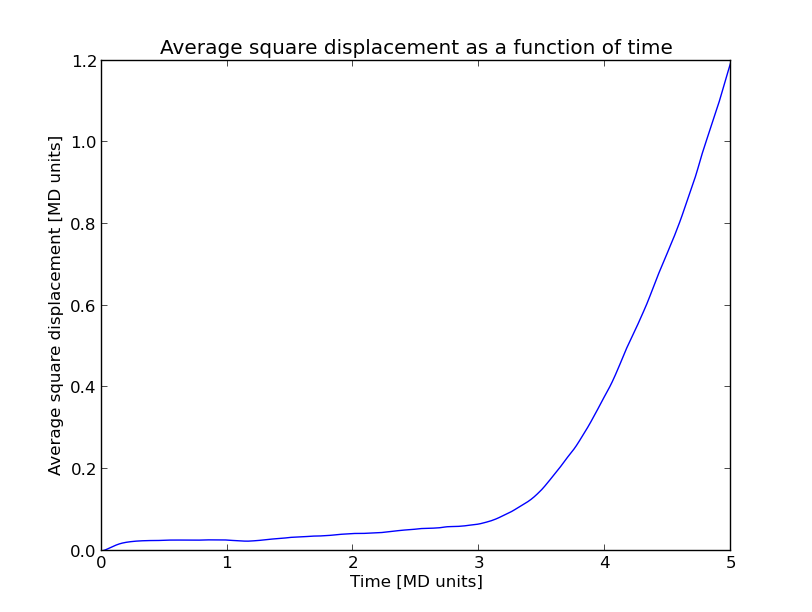
\includegraphics[width=7cm]{phasetransdist.png}
	\label{fig:subfig23}
}
\caption[Optional caption for list of figures]{The figures show \ref{fig:subfig13} the pressure as a function of temperature in a system that is linearly heating up, and \ref{fig:subfig13} the mean square displacement. The fact that the mean square displacement starts increasing at the same time as the sudden increase in pressure points to a phase transition from solid to liquid.}
\label{fig:9}
\end{figure}


\subsection{The diffusion constant}
We want to characterize transport in a fluid by measuring the self-diffusion of an atom: We give an atom $i$ a label, and measure its position as a function of time $\rvec_i(t)$. We find the diffusion constant from the mean square displacement of all atoms (we trace the motion of every atom):
\begin{equation}
 \langle r^2(t) \rangle = {1 \over N}\sum_{i=1}^N (\rvec(t) - \rvec_{\text{initial}})^2
\end{equation}
From theoretical considerations of the diffusion process we can relate the diffusion constant in the liquid to the mean square displacement through:
\begin{equation}
 \langle r^2(t) \rangle = 6Dt \text{ when } t \rightarrow \infty
\end{equation}
The average square displacement is plotted as a function of time in figure \ref{fig:10} for a starting temperature of 700 Kelvin (which gave an equilibriated temperature of around 320 Kelvin). We see a clear linear tendency, and we can measure $D$ to be roughly $D \approx 0.059$ in MD units.

  \begin{figure}
\centering
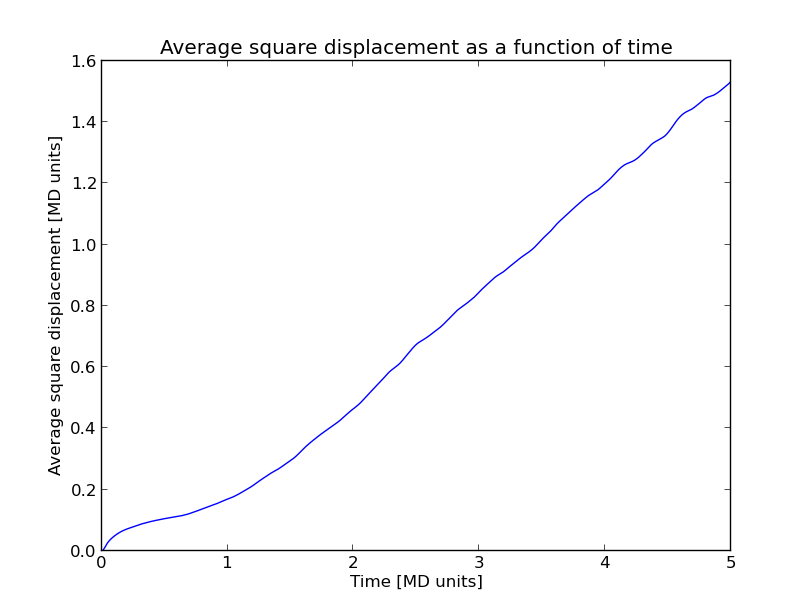
\includegraphics[width=10cm]{avgsqdisp.png}
\caption{\label{fig:10} The figure shows the avg square displacement as a function of time in liquid Argon.}
\end{figure}

\subsection{Microscopic structure - radial distribution functions}
The radial distribution function $g(r)$, also called a pair correlation function, is a tool for characterizing the microscopic structure of a fluid. It is interpreted as the radial probability for finding another atom a distance $r$ from an arbitrary atom, or equivalently, the atomic density in a spherical shell of radius $r$ around an atom. It is commonly normalized by dividing it with the average particle density so that $\lim_{r\rightarrow \infty} g(r) = 1$.

The results for a solid and a liquid is shown in figure \ref{fig:11}. We see that the case for a liquid looks smoother than that for a solid. This could be explained by the fact that there is a higher correlation between the particle positions in the solid (i.e. the particles are trapped in a grid).

\begin{figure}[ht]
\centering
\subfigure[radial distribution for a liquid]{
	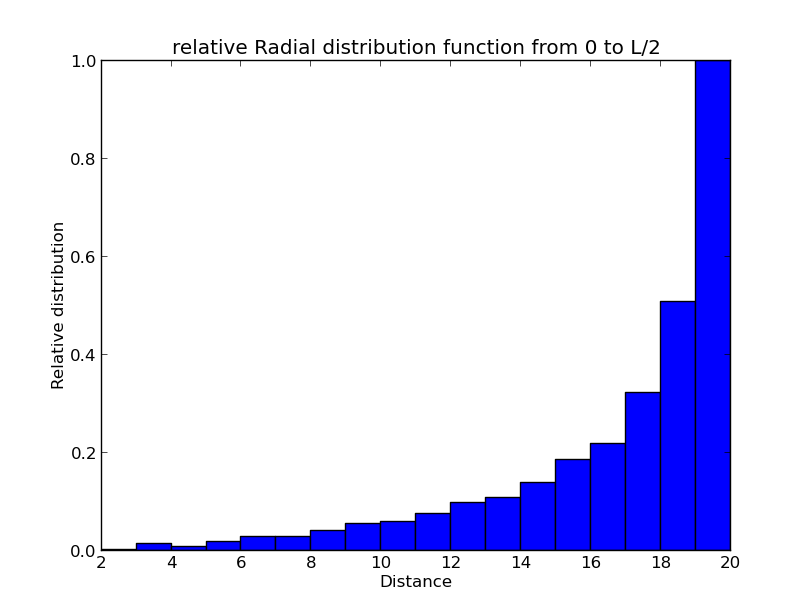
\includegraphics[width=7cm]{raddistgas.png}
	\label{fig:subfig12}
}
\subfigure[radial distribution for a solid]{
	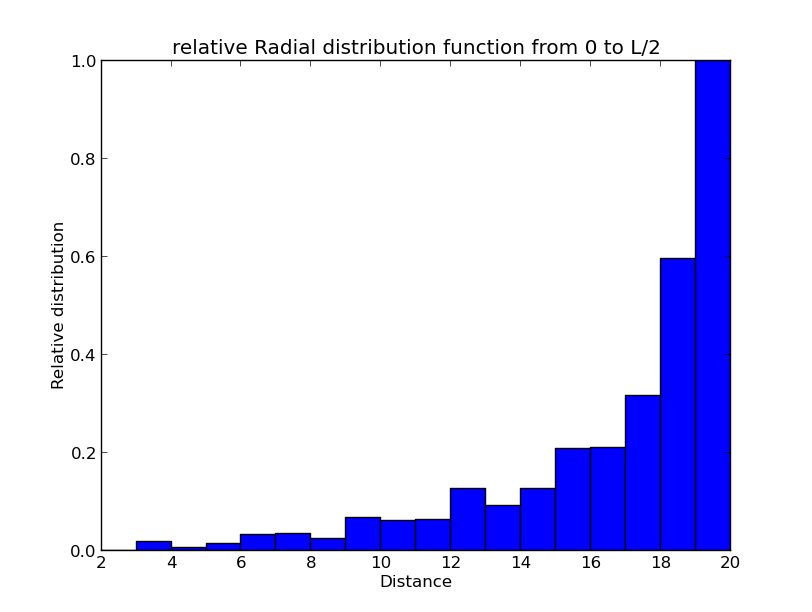
\includegraphics[width=7cm]{raddistsolid.png}
	\label{fig:subfig22}
}
\caption[Optional caption for list of figures]{The plots show the radial distribution for \label{fig:subfig12}, a liquid, and \label{fig:subfig22}, a solid}
\label{fig:11}
\end{figure}

\clearpage

\section{Thermostats}
In order to simulate the canonical ensemble, interactions with an external heat bath must be taken into account. Many methods have been suggested in order to achieve this, all with their pros and cons. Requirements for a good thermostat are: 
\begin{itemize}
 \item Keeping the system temperature around the heat bath temperature
 
 \item Sampling the phase space corresponding to the canonical ensemble 
 
 \item Tunability
 
 \item Preservation of dynamics
\end{itemize}
Here we will implement two thermostats; the Berendsen thermostat and the Andersen thermostat.

\subsection{The Berendsen thermostat}
Many thermostats work by rescaling the velocities of all atoms by multiplying them with a factor $\gamma$. The Berendsen thermostat uses 
\begin{equation}
 \gamma = \sqrt{1 + {\Delta t \over \tau}\left( {T_\text{bath} \over T}  - 1 \right)}
\end{equation}
with $\tau$ as the relaxation time, tuning the coupling to the heat bath. Though it satisfies Fourier's law of heat transfer, it does a poor job at sampling the canonical ensamble. If we set $\tau = \Delta t$, it will keep the estimated temperature exactly constant. It should be put to 10-20 times this value. The resulting temperature is shown in figure \ref{fig:12}. We see that after the usual dip, the temperature increases to the thermostat value (here set equal to the initial value of the system).

  \begin{figure}
\centering
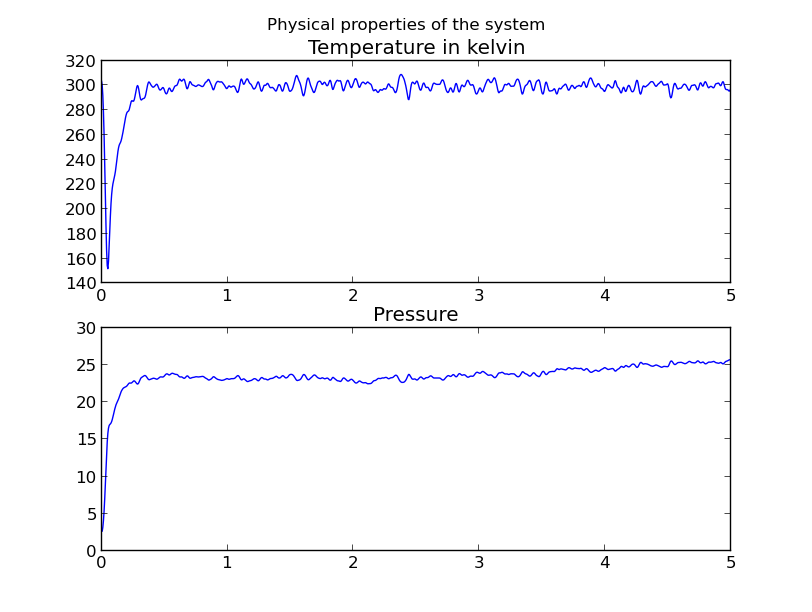
\includegraphics[width=10cm]{berendsenthermostat.png}
\caption{\label{fig:12} The figure shows the temperature of the system when controlled by a Berendsen thermostat at 300 Kelvin.}
\end{figure}

\subsection{The Andersen thermostat}
The Andersen thermostat simulates (hard) collisions between atoms inside the system and in the heat bath. Atoms which collide will gain a new normally distributed velocity with standard deviation $\sqrt{k_B T_\text{Bath}/m}$. For all atoms, a random uniformly distributed number in the interval [0,1] is generated. If this number is less than $\Delta t / \tau$, the atom is assigned a new velocity. In this case, $\tau$ is treated as a collision time, and should have about the same value as the $\tau$ in the Berendsen thermostat. The Andersen thermostat is very useful when equilibriating systems, but disturbs the dynamics of e.q. lattice vibrations.

The resulting temperature function when using the same parameters as for the Berendsen thermostat is shown in figure \ref{fig:13}.

  \begin{figure}
\centering
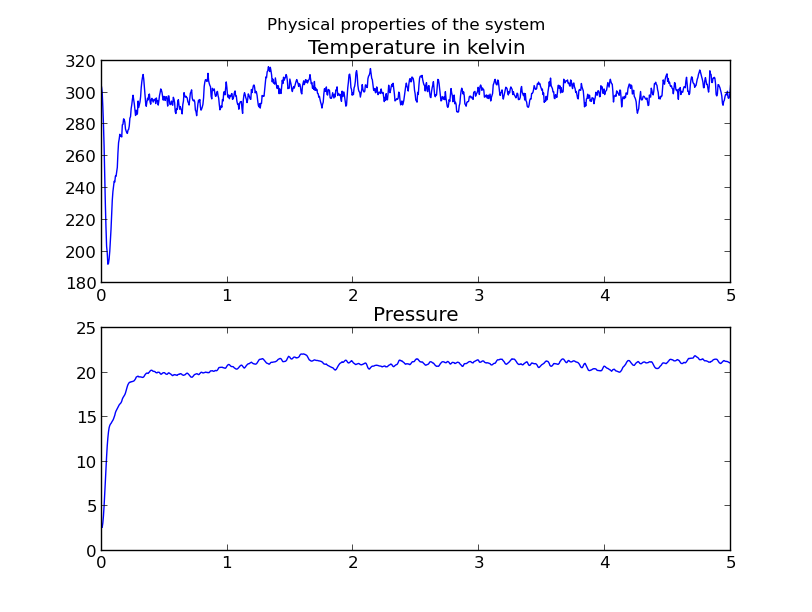
\includegraphics[width=10cm]{andersenthermostat.png}
\caption{\label{fig:13} The figure shows the temperature of the system when controlled by a Andersen thermostat at 300 Kelvin.}
\end{figure}
 \end{document}